\documentclass[11pt]{article}
\usepackage[margin=1in]{geometry}
\usepackage{amsmath}
\usepackage{booktabs}
\usepackage{tikz}
\usepackage{array}

\title{Assignment 2: Design Your Dream Logo \\ \large Logo Name: \textbf{Nimbus}}
\author{Aishwarya J S}
\date{August 6, 2026}

\begin{document}
\maketitle

\section*{Concept}
\textbf{Nimbus} is an imaginary weather-forecasting app. The logo shows a sun rising
behind a three-puff cloud, sitting above a rolling green horizon with two small
mirrored hills and gentle wind lines. The whole design is built around a single
\textbf{vertical mirror axis} ($x=0$): every element on the right has a matching
mirrored twin on the left.

\section*{Equations Used (15 total)}

\begin{center}
\begin{tabular}{@{}clll@{}}
\toprule
\# & Equation (Desmos syntax) & Type & Represents \\
\midrule
1  & $x^2+(y-5)^2=2.25$                              & Circle              & Sun boundary \\
2  & $x^2+(y-5)^2 \le 2.25$                            & Circle (inequality) & Sun fill (color) \\
3  & $x=0,\ \{6.5\le y\le 7.2\}$                       & Linear              & Sun ray, top \\
4  & $y=x+5,\ \{1.6\le x\le 2.1\}$                     & Linear              & Sun ray, upper-right \\
5  & $y=-x+5,\ \{-2.1\le x\le -1.6\}$                  & Linear              & Sun ray, upper-left (mirror of \#4) \\
6  & $(x+1.5)^2+(y-1)^2=0.81$                          & Circle              & Cloud puff, left \\
7  & $x^2+(y-1.3)^2=1.69$                              & Circle              & Cloud puff, center \\
8  & $(x-1.5)^2+(y-1)^2=0.81$                          & Circle              & Cloud puff, right (mirror of \#6) \\
9  & $y=0.3,\ \{-2.4\le x\le 2.4\}$                    & Linear              & Cloud base line \\
10 & $x^2+(y-1.3)^2\le1.69\ \{y\ge0.3\}$               & Circle (inequality) & Cloud fill (color) \\
11 & $y=0.15x^2-3.5,\ \{-3.2\le x\le 3.2\}$            & Quadratic           & Rolling horizon \\
12 & $y=-0.6|x+1.8|-2.5,\ \{-2.7\le x\le -0.9\}$        & Absolute value      & Hill, left \\
13 & $y=-0.6|x-1.8|-2.5,\ \{0.9\le x\le 2.7\}$          & Absolute value      & Hill, right (mirror of \#12) \\
14 & $y=0.12\sin(4x)-1.7,\ \{-2.6\le x\le -0.4\}$       & Trigonometric       & Wind gust, left \\
15 & $y=0.12\sin(4x)-1.7,\ \{0.4\le x\le 2.6\}$         & Trigonometric       & Wind gust, right (mirror of \#14) \\
\bottomrule
\end{tabular}
\end{center}

\noindent Five function types appear: \textbf{linear, quadratic, circular, absolute
value, and trigonometric}. Inequalities (\#2, \#10) shade the sun and cloud with
color instead of leaving them as outlines. Symmetry is clearly visible: equations
\#4/\#5, \#6/\#8, \#12/\#13, and \#14/\#15 are each mirror pairs reflected across the
vertical axis $x=0$, so the logo looks identical if flipped left to right.

\section*{Mathematics Behind the Design}
The logo relies on reflective symmetry rather than rotational symmetry, which is
achieved simply by pairing every off-center equation with a version whose
horizontal shift has the opposite sign -- for instance $(x-1.5)^2+(y-1)^2=0.81$
mirrored to $(x+1.5)^2+(y-1)^2=0.81$ for the cloud puffs, and $|x-1.8|$ mirrored to
$|x+1.8|$ for the hills. The three cloud circles overlap so their union reads as a
single soft cloud shape, while the inequality $x^2+(y-1.3)^2\le1.69$ restricted to
$y\ge0.3$ fills only the puff above the cloud's flat base, avoiding an ugly circular
bottom edge. The quadratic horizon curves gently upward on both sides since its
coefficient is positive, giving a natural "bowl" shape for the ground, and the two
absolute value hills sitting on it use $|x-c|$ shifts to place identical V-shaped
peaks symmetrically without duplicating the underlying math. The sine-based wind
lines were chosen over straight lines specifically to suggest motion and air,
something no polynomial or absolute value function can convey as naturally.

\section*{Preview (TikZ reconstruction of the Desmos graph)}
\begin{center}
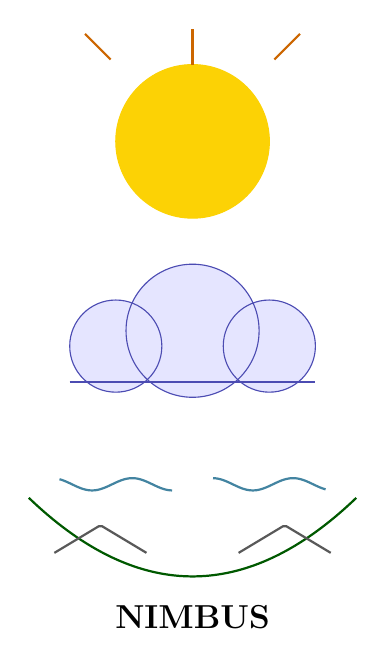
\begin{tikzpicture}[scale=0.65]
  \filldraw[yellow!70!orange] (0,5) circle (1.5);
  \draw[orange!80!black, thick] (0,6.5) -- (0,7.2);
  \draw[orange!80!black, thick] (1.6,6.6) -- (2.1,7.1);
  \draw[orange!80!black, thick] (-1.6,6.6) -- (-2.1,7.1);

  \filldraw[blue!10] (-1.5,1) circle (0.9);
  \filldraw[blue!10] (0,1.3) circle (1.3);
  \filldraw[blue!10] (1.5,1) circle (0.9);
  \draw[blue!40!gray] (-1.5,1) circle (0.9);
  \draw[blue!40!gray] (0,1.3) circle (1.3);
  \draw[blue!40!gray] (1.5,1) circle (0.9);
  \draw[blue!40!gray, thick] (-2.4,0.3) -- (2.4,0.3);

  \draw[green!35!black, thick, domain=-3.2:3.2, samples=60, smooth, variable=\x]
    plot ({\x},{0.15*\x*\x-3.5});

  \draw[gray!70!black, thick, domain=-2.7:-0.9, samples=30, smooth, variable=\x]
    plot ({\x},{-0.6*abs(\x+1.8)-2.5});
  \draw[gray!70!black, thick, domain=0.9:2.7, samples=30, smooth, variable=\x]
    plot ({\x},{-0.6*abs(\x-1.8)-2.5});

  \draw[cyan!60!black, thick, domain=-2.6:-0.4, samples=60, smooth, variable=\x]
    plot ({\x},{0.12*sin(4*\x r)-1.7});
  \draw[cyan!60!black, thick, domain=0.4:2.6, samples=60, smooth, variable=\x]
    plot ({\x},{0.12*sin(4*\x r)-1.7});

  \node[font=\bfseries\large] at (0,-4.3) {NIMBUS};
\end{tikzpicture}
\end{center}

\end{document}